\documentclass[11pt]{article}
\usepackage{natbib}
\usepackage{amssymb}
\usepackage{amsmath}
\usepackage{fullpage}
\usepackage{setspace}
\usepackage{graphicx}
\usepackage{array}
\usepackage{tabularx}
\usepackage{verbatim}

\title{Improved Ranking through Black Box Testing}
\author{Jesse Welch}
\date{May 2012}

\doublespace
\begin{document}
\maketitle

\tableofcontents
\newpage

\section{Introduction}
Black box testing is a useful method for diagnosing faults within a program. Rather than having to read through source code to find flaws, black box testing allows a set of failures to be presented without any detailed knowledge required.

When a set of black box tests are run on multiple solutions to a single problem, more information is available. Not only do we have the test results, but we have an ability to compare the test results. We can use this ability to find redundant tests, and limit the amount of noise shown for each solution. We can also use this information to compare the solutions, ranking them based on functional correctness.

Prior work demonstrates methods for both ranking and reducing redundant tests. In this paper, we will improve upon these methods in several ways. We will demonstrate a method for improving the ranking function by allowing additional results. We will introduce a method for allowing the ranking algorithm to continue to function with incomplete results. We will introduce a novel algorithm for performing additional noise reduction on each individual solution. Finally, we will introduce an infrastructure designed to make further algorithmic improvements and reduction strategies simple to implement.

\section{Ranking Solutions}
\subsection{The Algorithm}
When presented with the black box test results of many solutions to the same problem, one of the simplest and most useful things to do is to rank the functional correctness of the solutions. Naive algorithms for this perform poorly. For example, ranking solutions based on the percentage of tests that pass is extremely biased, frequently ranking solutions with a single, easy to test flaw as less correct than solutions with multiple, difficult to test bugs.

Claessen et. al. demonstrated an algorithm that is a substantial improvement \cite{Claessen}. They created large test suites automatically using QuickCheck \cite{QuickCheck}, and as a result, most of their tests were entirely equivalent. Rather than considering each test result as equally informative and comparing based on the results of every test run, they partitioned the tests into equivalence classes.

\centerline{ Given tests $T_O$ and $T_1$ and solution set $S$}
$$ T_0 \equiv T_1 \iff \forall s \in S s(T_0) \equiv s(T_1) $$

Using this example, a test set $T$ could be reduced into a set of its equivalence classes. From these equivalence classes, a single representative example could be drawn, creating a new test set $T\prime$. This step alone substantially improves the validity of the ranking algorithm. Ranking students based on the percentage of tests passed in $T\prime$, a solution with a single flaw will rank higher than a program with multiple flaws, regardless of how easy they are to test.

However, this method is still limited, and still has its own biases. For example, in some solutions, a single flaw will cause the failure of multiple equivalence classes of tests, causing the flaw to look worse than a seemingly equivalent flaw in a different program. And in general, we are still create a direct ranking of solutions whose failures may come in completely different sections of the problem, and thus be truthfully incomparable.

This general flaw is a consequence of the fact that a true ranking algorithm creates a total order of the solutions. When utilizing a percentage based metric, for every pair of solutions, one must be more correct, or they are equivalent. However, sometimes solutions are truly incomparable. For example, a problem may contain two subproblems, each of them entirely distinct. If one solution fails tests only on the first subproblem, and a second solution fails only on the second subproblem, they are truly incomparable. Claessen's algorithm allows for a "ranking" that represents this fact. In lieu of an artificial total order of solutions, Claessen's algorithm creates a partial order. It does this using a binary representation of results, tests are either passed or failed. These results are equal to themselves, and PASS $>$ FAIL.

\centerline{Given solutions $S_1$ and $S_2$, and test set $T$}
$$S_1 \equiv S_2 \iff \forall t \in T S_1(t) = S_2(t)$$
$$S_1 > S_2 \iff \forall t \in T S_1(t) \geq S_2(t) \wedge \exists t \in T \Rightarrow S_1(t) \neq S_2(t)$$


Under this definition, there are 4 possible results for comparing two solutions, $S_1$ and $S_2$. $S_1 < S_2$, $S_1 > S_2$, $S_1 = S_2$, or $S_1$ and $S_2$  are incomparable. This definition gives us every possible relationship between the solutions, rather than the 3 possibilities presented by a percentage based ranking. Additionally, it removes any biases based on the \emph{number} of tests failed. Instead, it is based only on the relationship between failed tests---anomalous failure counts will not affect the ranking.

Using this algorithm, we are able to successfully create accurate rankings of different student solutions.

\begin{figure}
\centering
\includegraphics{rank1.ps}
\caption{Edges point from a functionally inferior solution to a functionally superior one. "|" represents a class of tests passed by the equivalence class, "." represents a class of tests failed by the equivalence class.}
\end{figure}


\subsection{Adding More Outcomes}
The Claessen algorithm is based upon a simplification of the result of a black box test set. While it is true that without looking into the source code, the only thing we know about a solution is its test results, it is not true that these results are limited to a binary PASS/FAIL. In truth, we have much more information than this. A test can be passed, or it can be failed in any  number of ways. It may segfault. It may throw an exception. It may produce an incorrect result. The number of potential test results is not arbitrarily limited, and so we may be able to find further information by not limiting our algorithm's analytical powers to an imposed binary.

Claessen's algorithm needs extremely minimal extension in order to allow for non-binary outcomes. We need not change anything except what $>$ means. This step, however, presents an interesting problem. When allowing only binary outcomes, the total order of outcomes is self-evident: PASS$>$FAIL. When dealing with non-binary outcomes, however, there is no readily available ordering. Is an error that crashes the process ``better'' than one that silently produces wrong answers? In some cases, the process should be kept running at all costs. In others, the increased visibility of a catastrophic failure may be preferred to the subtle incorrectness of a wrong answer. In truth, the ranking of these outcomes is a subjective decision.

Since no universally correct ranking of outcomes is possible, we chose to examine what would happen if the algorithm was extended by a ranking determined by subjective choice. If we find a more representative ranking under one arbitrary ordering of outcomes, a different ordering should produce a ranking that is equally more representative to a different subjectivity. To this end, we imposed an arbitrary total order. The ordering was simple: PASS$>$INCORRECT$>$FAILURE, where FAILURE is defined as an error that brings down the process/interpreter. We chose this ordering because our datasets represent student solutions, and the students were told that a segmentation fault (or related fatal error) would result in a 0\% as their grade on functional correctness.


\begin{figure}
\centering
\includegraphics[scale=0.5]{rank1.ps}
\includegraphics[scale=0.5]{rank2.ps}
\caption{The first graph was created using binary outcomes, the second using multiple outcomes.}
\end{figure}

Using our new comparison function (but an algorithm unaltered from Claessen's), we found several interesting properties. First, in most cases, the additional outcomes made no difference. This was a surprising fact, and shows that the equivalence classes produced by the algorithm demonstrate a stronger degree of relatedness than previously known. Not only are these solutions getting the same binary results for every test, they are, in many cases, failing in  identical ways. Equivalence classes of solutions generally document programs that are \emph{extremely} similar.

(side by side where new comparison function harms)

In several of our datasets, we found that the additional outcomes did not improve the ranking graph, but in fact made it less descriptive. Rather than ranking solutions that were previously considered equivalent, as we hoped it would, we found that instead solutions that were originally considered equivalent were now considered incomparable.

(side by side where new comparison function works)

However, in some cases, the new comparison function was effective, successfully ranking solutions that were previously deemed equivalent. This new ranking is a strongly positive effect, improving our comprehension of the relationship between solutions. However, the potential for negative effects looms large. There exists a potential use for the new comparison function which mitigates the negative effects while retaining the positive ones. If we first apply the Claessen algorithm with the original comparison function, we will get a set of equivalence classes based upon the binary results. We can then see if we can make these classes more descriptive by applying the algorithm with the multiple outcomes comparison function to each equivalence class. If the solutions are ranked, we keep the result, replacing the rankings from the original comparison with those from the new. If the solutions are rendered incomparable, we keep the original comparison. And if there is no change, we can do either. In this way, the new comparison function can be used in concert with the original to create rankings which are either equal to those created with only the original, or strictly superior.

\subsection{Limiting the Test Set}

The computational power required to adequately test a program can frequently be substantial. To fully exercise even a medium-scale program, thousands of unit tests (potentially generated from hundred of QuickCheck properties) may be required. Some or all of these tests may be expensive to run. A test that induces an infinite loop will run until an arbitrarily long timeout point. A test that does not induce an infinite loop may simply take a long time to run, or allocate large blocks of memory.

Running a test set can therefore be very expensive, particularly upon many solutions. Each expensive test needs to be run for each solutions, and a particularly poor solution may cause many tests to loop infinitely. It would therefore be useful to not run the entire test set on every solution. 

We found running the entire test set for each student prohibitively expensive. If we needed to run each test on each solution we needed to spawn a new process for each test, for each solution. Running a test set of ~1000 tests with this method of testing took ~4 hours of CPU time per student. This became even more severe of an issue when accounting for the fact that tests sets generally need to be debugged, and 4 hours of CPU time was simply unacceptable.

Instead, we chose to test the solutions using block testing. Rather than spawning a new process for each test for each solution, we spawned a process for each block of related tests. If any of these tests brought down the entire process, results for any tests which were not yet reported were simply not reported. Instead, they received a new, implicit outcome: Did Not Run (DNR).

With these new outcomes ``in'' our dataset, we were faced with the challenge of ranking based on them. There were two possible paths for ranking these solutions. The first would be to simply use the process described in the previous section, and extend the comparison function to place DNR arbitrarily within the ordering (perhaps as the worst result, or equivalent to a fatal error). This result produces useful rankings, but it forces us to limit what a DNR can mean.

The tester running the test set may choose to omit tests from a given solution for any number of reasons. Perhaps tests are omitted for the reasons we used, because a previous test caused a fatal error. But perhaps thy are omitted for a more positive reason. A tester could choose to start a portion of a test set by running an extremely difficult test set, one which simultaneously exercised every feature that portion is testing. If this test is passed, they may then choose to not run all of the simpler test cases, because they know the solution will pass them. And perhaps the tester eliminates some tests for each of these reasons, on the same test. In this case, there is no proper place for DNR in the ordering of outcomes. It could mean either PASS or FAIL, and so cannot be placed as better, worse, or equivalent to any of tehm.

In this case, we can choose another method for handling DNR outcomes. The procedure is very simple. We ignore them.

\centerline{Given solutions $S_1$ and $S_2$, and test set $T$}
$$S_1 \equiv S_2 \iff \forall t \in T where S_1(t) \neq DNR \wedge S_2(t) \neq DNR \wedge S_1(t) \equiv S_2(t)$$
$$S_1 > S_2 \iff \forall t \in T where S_1(t) \neq DNR \wedge S_2(t) \neq DNR \wedge S_1(t) \geq S_2(t) \wedge \exists t \in T \Rightarrow S_1(t) \neq S_2(t)$$
Two solutions are compared only on the tests for which each of them ran. In this way, we do not invalidate any of the possible meanings of DNR. In a properly deterministic test set, two solutions cannot differ only on tests for which one of them received a DNR. Instead, a prior test result must have \emph{caused} the DNR in one solution and not the other, and on this test they can still be compared. 

In the first situation previously discussed, in which a block of tests may not be run because a prior test crashed the block, solutions would differ on whether or not they ran the block, but the one which ran the block would also have an inherently better result---it passed the test which crashed the block. The solutions can be properly compared on this test.

In the second situation previously discussed, in wehich a block of tests may not be run because a prior test had a successful result, solutions would differ on whether they ran the block, but also on the initial test---the solution which did not run the block has an inherently better result---it passed the test which caused the block to not run. The solutions can be compared on this test.

Using this process, solutions can be compared whenever tests are not run, for whatever reason they are not run, as long as the reasons are deterministic. If tests are not run for a reason, we can still compare the solutions, based solely on the reason, \emph{without information loss}.

\section{The Implication Graph}
\subsection{Creating the Graph}
Black box testing data contains a wealth of information. Most obvious is the information about solutions, which we use to rank these solutions. But also present in the data is information about the tests themselves. This data can be used to improve the ranking algorith, but it also can be used towards an entirely new end: discovering the structure of the problem itself. The testing data contains information about the relationship between tests, but taken in the aggregate, this can be used to find information about the entire problem. Perhaps we can find several subcomponents of a problem whose constituent parts were poorly understood, or find relationship between known components that were considered independent.

A difficulty lies in the fact that to solve the general problem of discovering a problem's structure, we have to treat not just the solutions, but the problem itselfm, as a blackbox. When presented solely with the outcomes of a set of tests, we cannot try to buoy known information about the problem's structure, but instead must rediscover this structure, and hopefully new pieces of information as well. This creates a useful for of self-validation: if any known constituent parts are not discovered, the structure is likely incorrect.

We have attempted to diagram a problem's structure using implications between test outcomes. An implication is defined as follows:

\centerline{Given solution set $S$ and outcomes $O_1$ on test $T_1$ and $O_2$ on test $T_2$}
$$O_1 \Rightarrow O_2 \iff \forall s \in S where s(T_1) = O_1, s(T_2) = O_2$$

Using this definition, we attempt to discover every implication in the dataset. First we create a proposition for every outcome, and its inverse, on every test. Then we look for an implication (in either direction) between each pair of propositions. This is a $O(n^2)$ process, and so it is not computationally efficient to perform it on every test in the test set. However, by limiting to one test from each equivalence class of tests, n remains small enough to proceed.

This process is simplified even further by usage of a variation of the partitioning algorithm used to create the equivalence classes of tests. Rather than partitioning the tests, we partition the \emph{propositions} into equivalence classes. For a given solution, a proposition is considered true if it holds on that solution (e.g. the proposition Test 2 PASS hold for a solution if it passes Test 2), and false if it does not hold. Two propositions, $P_1$ and $P_2$, are considered equivalent if they hold for the exact same set of solutions.
$$P_1 \equiv P_2 \iff \forall s \in S, P_1(s) = P_2(s)$$
Now, rather than having to find implications between every proposition, we need to find them between every \emph{class} of propositions.

The set of implications within a dataset forms a natural structure: a directed graph. Each class of propositions is a node in the graph, and each implication is an edge from the implicating proposition to the implicated.


(example of a toy implication graph)


Given this implication graph, the question remains: Does it actually diagram the problem's structure? We were provided with a natural experiment to begin to test this question. Our students were given an assignment that contained 14 problems. Each of the problems was entirely self-contained, and there was no code overlap between the problems. Some problems covered related topics, and so relic relationships might appear in the data, but by and large, we expected these problems to be diagrammed as entirely separate components.

(divtest implication graph, with subproblems boxed in - this can probably be improved)

The results of this experiment were mixed. We did not find that every subproblem made an entirely separate subgraph, but instead that the subproblems made subgraphs that were sometimes connected, with implications between portions of the problem that should not be possible in the underlying problem.

\subsection{Improving the Visualization}
The implication graph, as produced contains all of the information about implications contained within the dataset. It also contains large amounts of tautological information, implications which are true regardless of the dataset. These tautologies are represented both as edges within the graph and as equivalences within a single node.

These tautologies are generally relationships between propositions that work on the same test. If a test $t$ fails, $t$ did not pass; if $t$ does not run, $t$ did not fail, etc. Informing the person analyzing the implication graph of these relationships adds nothing to the structure of the problem, it merely dilutes the relevant relationships. Though removing these tautologies removes information from the graph, it is not information that an intelligent viewer will not readily assume.

There are two processes necessary for removing tautologies from the implication graph, one if they are within a single node, another if they are between nodes. Removing an intranode tautology is simple. One of the two tautologically propositions is simply removed from the node, leaving only one member of the pair. In our implementation, we attempted to retain the more precise proposition (PASS is more precise than NOT FAIL, because it describes only one outcome and not a set). 

Removing internode tautologies is equally simple, though more likely to confuse the viewer. Any of the relationships between two equivalence classes of propositions is tautological, we remove the edge in the graph. This relationship can still be assumed by an intelligent viewer, because the tautology remains self evident. However, the relationships between the other members of the equivalence classes have now become implicitly documented, rather than explicitly.

Also present in the implication graph is an entire class of redundant relationships. For two related propositions, $A$ and $B$, two implications are created: $A \Rightarrow B$ and $\neg B \Rightarrow \neg A$. This is true for two equivalence classes as well, the negation of a class being the negation of each of its members. Given one of these implications, the existence of the other is tautological. Therefore, we can include only one of them, without suffering information loss to an intelligent viewer. A difficulty in implementation lies in choosing a subset of these implications that leaves a minimal number of nodes in the final graph.

Intelligent viewers may choose whether or not performing any of these reductions on the implication graph increases clarity by limiting the amount of information displayed, or reduces clarity by rendering some relationships implicit. Nonetheless, it is clear that performing these reductions causes a substantial reduction to the size of the resulting implication graph.

(side by side of an ugly graph pre-reduction and a prettier graph post reduction.

\section{Noise Reduction on Test Sets}
\subsection{Claessen's Algorithm}
In Claessen's paper on ranking, there are several forms of noise reduction already performed. The first is the fundamental step of the algorithm, in which tests are grouped into equivalence classes. This step alone reduces from the original number of tests to a substantially smaller subset. Even with test sets numbering well into the thousands, this step never produced more than 144 equivalence classes during our experimentation.

After this large scale reduction, Claessen's algorithm contains another form of noise reduction. A test $T_0$ is redundant if

$$FAIL (T_0) \equiv FAIL(T_1) \cup FAIL(T_2)$$
where all three tests are drawn from different equivalence classes. This was justified with the argument that, rather than discovering a new faults of its own, $T_0$ likely provoked both of the faults discovered in $T_1$ and $T_2$. Removing $T_0$ therefore does not cause any information loss. Instead, its removal simplifies the test set to a smaller, but still representative sample of tests.

\subsection{Union*}
The logical basis to Claessen's algorithm that a test can be redundant because it provokes the flaws already demonstrated by two other non-redundant tests\cite{Claessen}, can be extended further. Why should we limit this to only circumstances where the flaws are in exactly two other tests? Why not any number? We propose an extended algorithm, one which removes any tests whose set of failures is equal to the union of the failures of \emph{any number of tests}. 

A test $T_0$ is redundant if

$$FAIL (T_0) \equiv FAIL(T_1) \cup FAIL(T_2) \cup ... \cup FAIL(T_n) $$

(if I managed to write the first proof, proving this the same shouldn't be hard)

A naive implementation of this algorithm is computationally complex. Given a set of tests $T$, we need to run the algorithm for each member $t$ of $T$, checking whether its failure set is equal to the union of any subset of tests in $T$ that does not contain $t$. This is simply too much work, so a different solution must be found.

Thankfully, the implication graph lends itself to a vastly simplified implementation. We do not need to check the union of every possible subset of tests, only the union of those that could possibly be useful. Using the implication graph, given a test $t$ and a test set $T$, we can easily find the subset $T\prime$ which only contains tests whose failures are a subset of $t$. Any test in $T$ but not in $T\prime$ cannot possibly contribute to an equal union, because it contains at least one failure not in $t$. Therefore, we can simply apply the algorithm once, to every member of $T\prime$. $t$ is redundant if $FAIL(t) \equiv \cup^* T\prime$.

\subsection{Comparison}
Union* must reduce at least as many tests as Claessen, and can reduce more. This is because every test that will be removed under Claessen will be removed under exactly the same conditions in Union* (the union of two tests is simply a specification of the union of any number of tests). In theory, Union* is capable of outperforming Claessen

\begin{figure}
\verbatiminput{testset}
\includegraphics{toy.ps}
\includegraphics{toyb.ps}
\caption{Graphs produced using test set above. First graph has been reduced using Claessen, the second Union*. Note that Test 4 has been successfully reduced by Union*}
\end{figure}

In practice, we discovered a different situation. On 10 different real world datasets (each dataset was the student submissions for a different assignment, drawn from two different courses), we found no difference between reduction performed by the Claessen algorithm and the Union* algorithm. This was a surprising result, and demonstrates several things. Trivially, it confirms that the Union* algorithm does no worse than Claessen. More substantially, we discovered that the Claessen algorithm is surprisingly powerful. In every tested real world case, the union of two tests was enough to remove every test that could be found redundant under union.

There are several potential explanations for this fact. One is that no test tests more than two underlying faults. This is extremely unlikely, as it is relatively simple to write a test that exercises large sections of a program's functionality, and can readily provoke more than two potential faults. Another possibility lies in the method of building tests. The test sets we use, being generally developed from QuickCheck properties, deliberately exercise a specific area of functionality \cite{QuickCheck}. Similarly, when hand written unit tests are allowed, they also generally exercise small areas of functionality, rather than the entire program. A different style of test design might allow Union* to have more success, removing large tests that attempt to exercise every possible fault in the program, when these faults are better demonstrated by small tests. A final possibility is that we simply don't have enough solutions, and that a greater diversity in solutions would increase the difference between the two algorithms.

\section{Noise Reduction on Witness Sets}
\subsection{The Algorithm}
There exists a minimal subset of tests which we must retain in order for the ranking algorithm to continue to function without information loss. This set of tests is not necessarily as small as the minimal number of tests needed to diagnose the failures in a single solution. There exist many situations in which multiple tests are needed to differentiate between the entire set of solutions, but a single representative test would be enough to diagnose the flaws of an individual solution.

All forms of noise reduction previously discussed rely on examining the relationships between the classes of solutions, and removing tests on which all members of a  class can be expected to perform the same. However, when attempting noise reduction at the granularity of a single solution, the relationships between solutions are not applicable. The only relationships relevant at this level  are those between the tests themselves.

The implication graph is a representation of the relationships between these tests. It presents many discoverable relationships (implies, implied by, reachable from, etc.). Using this graph, we are able to perform noise reduction at the level of a single solution, a novel process. For simplicity, we chose to examine only one of the available relationships, direct implication. Our algorithm is as follows:

\centerline{Given two tests $T_1$ and $T_2$ and solution $s$}
$$if s(T_1) = FAIL \wedge s(T_2) = FAIL \wedge FAIL(T_1) \Rightarrow FAIL(T_2), remove T_2$$

Given a perfect implication graph, in which every implication is not just found in the data but representative of the problem itself, this algorithm reduces the tests presented as  failed to the set of the easiest tests failed. 

If two tests are needed to differentiate the solutions on the solution class scale, it is possible (and frequently true), that one is simply an easier version of itself. For example, we ran our algorithms on a set of solutions to the problem of reducing the lambda calculus. Following all class level reductions, two tests were among those that remained:

\verbatiminput{lambdatests}

$T_1$ tests where a solution has implemented eta reductions at all. $T_2$ tests whether a solution has implemented eta reductions \emph{in a specific place}. $T_2$ was explicitly designed to be a harder version of $T_1$. If you did not implement eta reductions at all, you would fail both. If you implemented them, you would pass $T_1$, but might still fail $T_2$ if they were not functioning properly in the specific case.

Because the flaw in $T_1$ directly causes a failure in $T_2$, $FAIL(T_1) \Rightarrow FAIL(T_2)$. This led our algorithm to be able to reduce the witnesses to any solution who failed both tests, providing only the output from $T_1$.

\begin{figure}
\verbatiminput{lambdareduction}
\caption{Machine output for a successful reduction in which $T_2$ (nr403) was removed due to failure of $T_1$ (nr97)}
\end{figure}

\subsection{Validity of Reductions}

This algorithm is definitively  capable of performing reductions, but a questions remains: Are the reductions good? Reductions performed on the class level cannot change the class structure. Both the Claessen algorithm and the Union* algorithm cannot cause information loss. But the witness reductions can. Though implications have a theoretical underlyin structure, they are drawn from the underlying data available, and this data is frequently flawed. This can lead to reductions in a test can be removed based on an implication from a test which tested an entirely different separate feature.

A readily available example is the dataset used to confirm the implication graph. As we discovered earlier, when tests were run on functions whose implementations were entirely independent, the functions generally formed into groups in the  graph, but there were implications between the groups. Using this implication graph, we performed a witness reduction on each solution, in order to test how many of the reductions we considered to be valid. In order to simplify analysis, we did not try ot delve into the relationship between each test, but instead used a simple metric. If two tests test the same function, any reduction upon them is valid. If they test different  functions, any reduction on them is invalid.

\begin{figure*}
\begin{tabularx}{\linewidth}{@{}XX@{}}
\small\verbatiminput{goodreductions}
&
\small\verbatiminput{badreductions}
\\
\caption{Good reductions}&
\caption{Bad reductions}
\\
\end{tabularx}
\end{figure*}


After running this experiment, we found that the witness reduction strategy achieved moderate success. Out of 422 reductions, 62.5\% were deemed to be valid. However, this result is somewhat misleading. A large number of the invalid reductions were concentrated in the least correct solutions. By omitting the reductions obtained from the two least correct solutions, the percentage of correct reductions jumps to 76.7\%. While eliminating these students is not something that can truly be done in practice, it demonstrates that witness reduction is highly accurate for most students, and extremely inaccurate for a select few.

Using the same definition of implications, but with multiple outcomes, we found a very different result. There were only 112 reductions, all of them related to the qsort function, and every one of them was valid. This was a positive result, but the fact that reductions were not made on tests of any other functions makes these results suspect.

Any invalid reductions discovered represent a failure in the implication graph, as they are based on implications which are likely not valid to the problem itself, but simply to the dataset the reduction process was done on. If the implication graph perfectly represented the problem structure, every reduction based on it would be good. Therefore, the more correct we make the implication graph, the more correct we make the witness reduction.



\section{Improving the Implication Graph}



When building the implication graph, we do not have access to the structure of the problem itself, only a small sample of attempts to solve the problem and there results on tests of the problem. We have no oracle to tell us when the structure is correct. However, there are many properties about the relationships between tests that we can utilize to remove implications that cannot possibly be present in the problem itself, as well as removing implications that may be true, but the we do not have enough information  to claim.

One class of implications we can remove entirely are those between the failure of one test, and the passage of another. Every problem has a fully correct and a fully incorrect solution, one which passes every test, and one which fails every test. Based on this, the following proofs are possible.


Assumption: There exists a fully correct and fully incorrect solution to every problem.

Theorem: The passage of one test cannot imply the failure of another test in the full problem space.

Proof: Assume $PASS(T_1) \Rightarrow FAIL(T_2)$. This means that every solution that passes $T_1$ fails $T_2$. However, there exists the fully correct solution S. For all tests T, S(T) = PASS. Therefore S($T_1$) = PASS, and S($T_2$) = PASS, contradicting our assumption.

Theorem: The failure of one test cannot imply the failure of another test in the full problem space.

Proof: Assume FAIL($T_1$) $\Rightarrow$ PASS($T_2$). This means that every solution that fails $T_1$ passess $T_2$. However, there exists the fully incorrect solution S'. For all tests T, S'(T) = FAIL. Therefore S'($T_1$) = FAIL, and S'($T_2$) = FAIL, contradicting our assumption.


Based on these proofs, we can safely remove from the implication graph every implication between the passage of one test and the failure of another.

From similar logic, we can remove every implication either to or from a test with universal results. If every student passed a given test, then any result on any other test will logically imply this passage. However, there exists the fully incorrect solution, which by definition failed this test. Therefore these implications are by definition based on incomplete information, because they do not take into account the failure of this test. The inverse means we can do the same to a test which every student failed, based on the fully correct solution. Similarly, if no student passed a given test, the  test's passage will logically imply everything. But we cannot make implications  from this result (or a test with no failures) because the fully correct and incorrect solutions mean we are basing these implications on incomplete data.

There is one other reduction we can make to the implication graph, for somewhat different reasons than the previous reductions. We can remove implications that may hold true in th actual problem structure, because we do not currently have enough information to assume them. If a given test result is achieved only by members of a single equivalence class, any implications based on it can be removed, because they are based on too little information to generalize from.

We don't have enough information because, if an outcome is achieved only by a single class, it logically must imply every other result achieved by that class's solutions (because every solution that achieved that result achieved each other result). But we simply cannot claim that each of these results is directly implied by a single result. If we do, we claim that knowing a single fact about a solution means that we know everything about it. This is obviously untrue.

\subsection{The Results  of Reducing the Implication Graph}

These reductions of the implication graph were critical to our ability to implement witness reduction. The first several reductions insured we were not making any reductions based on clearly invalid implications. The final reduction, in which we do not allow implications based on unique outcomes, was particularly important. Based on this reduction, we were able to improve the output give larger and more representative witness sets to the affected solutions.

\begin{figure}
\verbatiminput{example.witness}
\verbatiminput{example3.witness}
\verbatiminput{example2.witness}
\caption{The first set of failures is unreduced, the second set is reduced without alteration, and the third is reduced using the improved implication graph}
\end{figure}

\subsection{Continuing Problems}

Despite these reductions, we were not able to fully stop the algorithm from making invalid reductions. Though the implication graph can assuredly be improved further, and the witness reductions therefore improved as well, it is unlikely that we will ever be able to make completely valid reductions for most problems. The reason for this is twofold: the number of solutions available is finite, and  real world solutions are strange.

The first problem is fairly clear. In order to find the full structure of a problem, we need to know every possible correct and incorrect solution to it, an infinite  number of solutions. Presented with a finite dataset, we can only approximate this structure, a fundamental limitation.

The second problem is far more insidious. When attempting to find the structure of a problem, it is expected that if a test tests some feature of a program, and that feature has a flaw, the test will uncover it. However, in the real world, programs do not behave nicely. There may be two flaws within a feature, which generally cause the feature to fail, but sometimes work together to cause it to succeed.

In real world programs, we do not find clean connections of components, failures that always occur in concert, features bein implemented in uniform ways. Real programmers have flaws present at every known edge case, and sometimes at edge cases that were unknown. Flaws interact in unexpected ways, and programs, when tested as a black box, are generally unpredictable.

Nonetheless, we have found that, on real world datasets, witness reduction based on our best approximation of the implication graph is good enough to produce positive results. Though the eccentricities of real programs often meant that reductions the seemed obvious were not made, and sometimes that invalid reductions were, the process generally proved successful, and should prove more successful as future improvements to the graph are made.

\subsection{Witness Expansion}

The end goal of witness reduction is providing the smallest possible set of tests that diagnose the faults of a solution. A related goal is providing a solution the most accurate diagnostic information possible. The implication graph can be used to achieve this goal by expanding the witness set, rather than reducing it.

When we believed two tests were related based on the implication graph, we removed the harder test, because the simpler one provided the diagnostic information. However, for a more successful solution, which passed the easier test but failed the harder one, we provide no evidence of this relationship. But this relationship is a very useful thing, because it provides increased specificity on exactly where the fault lies within the solution. Using a very similar formula to our witness reduction, we can provide the student with these relationships.

\centerline{We inform a solution $S$ which passed test $T_1$ but failed $T_2$ of there results on  $T_1$ iff}
$$ S(T_1) = PASS \wedge S(T_2) = FAIL \wedge FAIL(T_1) \Rightarrow FAIL(T_2)$$



\section{Future Work}
This paper utilized the implication graph in order to implement several forms of noise reduction. These are not, however, every form of noise reduction the graph can be used for. By documenting the structure of a problem, the implication graph makes it easy for a researcher to implement new reduction algorithms. For example, rather than removing tests whose failures are the union of the implying failures, we could remove any test whose failures are the intersection of the implied failures. Or any test where every outcome is implied by another test. There are many possible reduction algorithms, and with the infrastructure of the implication graph in place, these algorithms can be readily implemented.

The implication graph's utility is not limited to noise reduction, or to problems in which ranking solutions is a goal. The implication graph diagrams the structure of a problem, and knowledge of this structure allows us to analyze other problems as well. This is particularly intriguing for problems in which a fully correct solution is unlikely, and quality is judged on accuracy, such as machine learning problems. Knowledge of the structure of this problem might allow a researcher to discover sets of difficult cases which fail together, or to better understand how the machine algorithm works.


\section{Conclusion}
There already exist in the literature algorithms to rank programs based on black box testing results. These algorithms are successful, but they use only a subset of the information available. We have attempted to use as much of the information present as possible to improve the existing algorithms and create our own.

Our Union* algorithm uses more of the testing data available to build a generalization of the union based reduction strategy implemented in \cite{Claessen}. This strategy proved to have minimal effect on the number of reduced tests in practice, but is computationally simpler than the Claessen algorithm, once the infrastructure has been built.

Our witness reduction algorithm is an entirely novel form of noise reduction. Rather than reducing tests only for the entire set of solutions, this algorithm allows further reductions to take place for each individual solution, creating a smaller set of failed test cases from which the solution's creator can diagnose faults.

Most importantly, we have created a powerful infrastructure from which further methods of noise reduction can easily be implemented. Rather than having to redesign for each new algorithm implemented, the implication graph allows for new reduction algorithms to be quickly implemented, and for entirely new types of reductions to be tested.

\bibliographystyle{plainnat}
\bibliography{thesis}

\end{document}
